\section{Planificación, metodología y presupuesto}

En esta sección, se van a definir los componentes fundamentales en la gestión del proyecto que nos permitirá desarrollar una aplicación en Alexa para mejorar las habilidades cognitivas y sociales de los adultos mayores a través del entretenimiento en residencias y centros de día.

\subsection{Planificación temporal}

Se ha elaborado un calendario, marcando con colores los plazos (en días) de las distintas tareas y subtareas en las que se ha desglosado el proyecto (\autoref{fig:planning1} y \ref{fig:planning2}.

\begin{figure}[H]
	\centering
	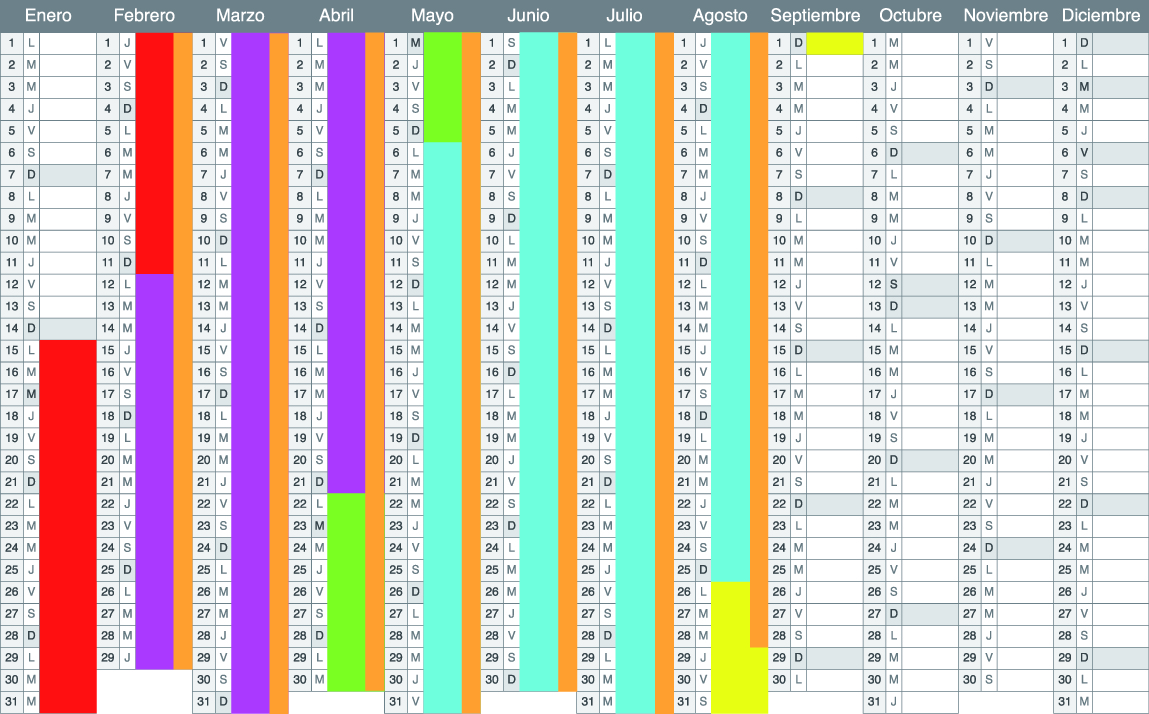
\includegraphics[width=1\textwidth]{imgs/tabla-planning1.jpg}
	\caption{Planificación temporal en el calendario}
	\label{fig:planning1}
\end{figure}

\begin{figure}[H]
	\centering
	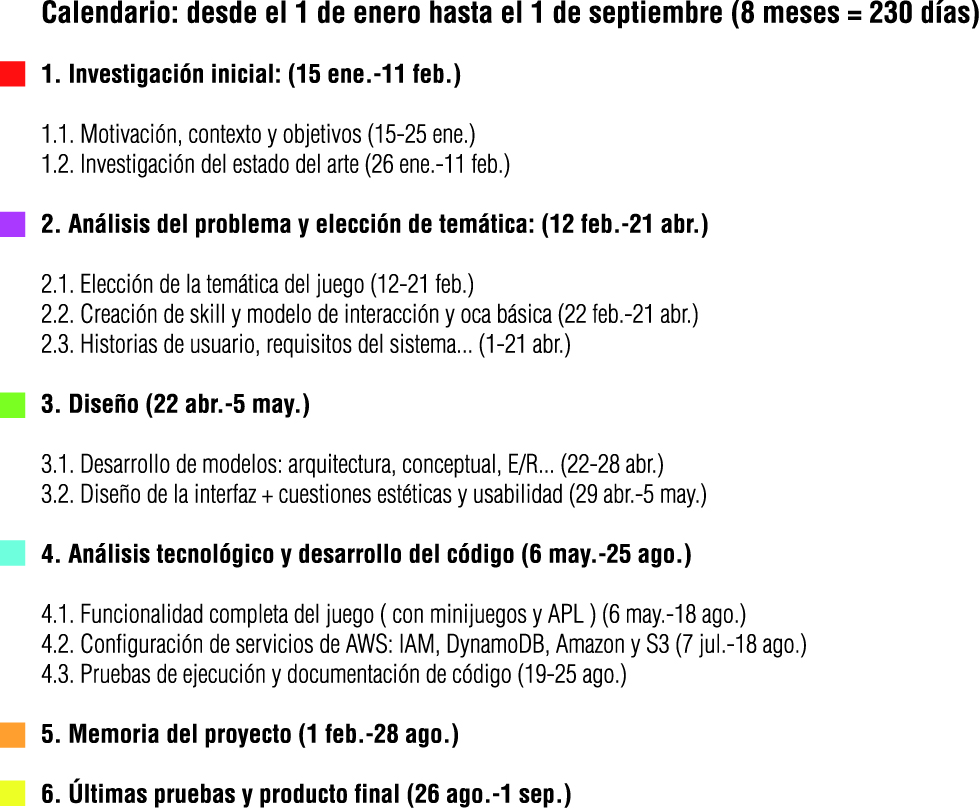
\includegraphics[width=1\textwidth]{imgs/tabla-planning2.jpg}
	\caption{Leyenda de la planificación temporal por (sub)tareas}
	\label{fig:planning2}
\end{figure}

Por tanto, si de esos 230 días que se ha estado trabajando en este proyecto, se estima que las horas empleadas cada día de media son 2'5, entonces se habrán dedicado cerca de 600 horas en total.

\newpage

\subsection{Metodología}

La metodología de desarrollo describe las técnicas y procesos que se seguirán para desarrollar el proyecto, incluyendo los roles y responsabilidades del equipo y los métodos de comunicación y gestión del proyecto. En este caso, se va a seguir un \textit{modelo evolutivo basado en prototipos} \parencite{carr1997prototyping}.

Este modelo incorpora el concepto de prototipos, entendidos como versiones preliminares del sistema que ayudan a refinar los requisitos y funcionalidades del mismo, mediante interacciones con los clientes y/o personas usuarias, antes del desarrollo del producto final.

En este caso, se tratará de un modelo evolutivo, ya que el enfoque se basa en ir construyendo y refinando una versión inicial del software en ciclos iterativos, adaptándose a los distintos cambios y necesidades hasta llegar a un producto final. La participación continua de los clientes y el carácter gradual del modelo permite flexibilidad a la hora de mejorarlo, y la posibilidad de definir requisitos no estáticos.

Todo modelo de prototipos se descompone en las siguientes fases, mostradas en la \autoref{fig:modelo-prototipos}:

\begin{figure}[H]
	\centering
	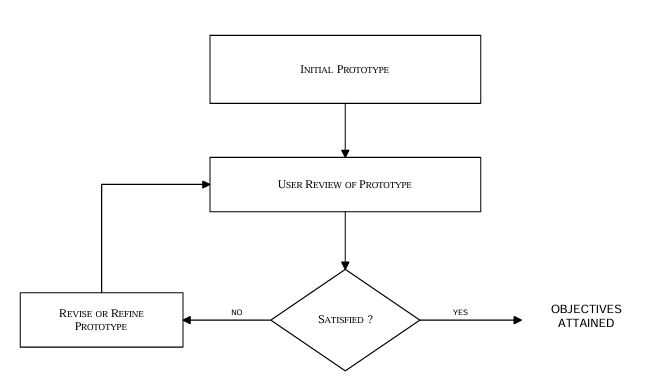
\includegraphics[width=0.8\textwidth]{imgs/modelo-prototipos.JPG}
	\caption{El proceso de desarrollo de prototipos \parencite{carr1997prototyping}}
	\label{fig:modelo-prototipos}
\end{figure}

\begin{enumerate}
    \item \textbf{Identificar los requisitos básicos}: previo al desarrollo de cualquier prototipo, se deben establecer las necesidades básicas en forma de requisitos funcionales, que pueden no estar completos del todo ya que se mejorarán en las siguientes fases.
    \item \textbf{Prototipo inicial}: se desarrolla una versión básica del software, centrándose en los aspectos relevantes de los requisitos establecidos anteriormente.
    \item \textbf{Revisión del usuario del prototipo}: los clientes y/o usuarios realizan pruebas sobre el prototipo, permitiendo detectar fallos o posibles mejoras en sus funcionalidades.
    \item \textbf{Revisión de requisitos y refinamiento}: en base a la retroalimentación de la fase anterior, se amplían o modifican las funcionalidades en una serie de ciclos iterativos, mejorando de forma gradual el prototipo inicial.
    \item \textbf{Aceptación/finalización}: una vez se ha terminado de revisar y refinar, se puede concluir que el prototipo satisface los requisitos establecidos, y por tanto, se ha logrado obtener el producto final.
\end{enumerate}


\subsection{Presupuesto}

El presupuesto permite gestionar los recursos del proyecto, desde el asignamiento de recursos humanos hasta la adquisición de equipamiento y materiales necesarios.

\subsubsection{Recursos humanos}
Los recursos humanos incluyen a las personas involucradas en el proyecto, tanto en las etapas previas al desarrollo como durante el mismo. 

Los datos de esta tabla han sido calculados a partir de las tablas salariales por titulación en España \parencite{glassdoor2024}.  

\begin{table}[H]
    \centering
    \begin{tabular}{|c|c|c|c|c|}
    \hline
    \rowcolor{lightgray}
    \textbf{Descripción} & \textbf{Horas} & \textbf{€/año} & \textbf{€/h} & \textbf{Coste (€)} \\
    \hline
    Desarrollador(a) de software & 300 & 33.750 & 16,23 & 4.869 \\
    \hline
    Ingeniero/a de Cloud Computing & 72 & 42.507 & 20,44 & 1.471,68 \\
    \hline
    Psicólogo/a & 10 & 23.794 & 12,20 & 122 \\
    \hline
    Expertos en Gerontología de la UGR & \multicolumn{4}{|c|}{Colaboración voluntaria} \\
    \hline
    \textbf{Total} & \textbf{382} & \multicolumn{2}{|c|}{} & \textbf{6.462,68} \\
    \hline
    \end{tabular}
    \caption{Presupuesto para recursos humanos}
    \label{tab:presupuesto-personal}
\end{table}

\subsubsection{Hardware}
La parte de hardware son todos los dispositivos físicos y electrónicos necesarios para llevar a cabo la aplicación.

El coste mensual del dispositivo se calcula dividiendo el precio original entre su vida útil (en meses), y después esa cantidad se puede multiplicar por el número de meses que se ha utilizado para hallar el importe amortizado.

\begin{table}[H]
    \centering
    \begin{tabular}{|c|c|c|c|c|}
    \hline
    \rowcolor{lightgray}
    \textbf{Descripción} & \textbf{Precio (€)} & \textbf{Vida útil (meses}) & \textbf{Uso (meses)} & \textbf{Importe amortizado (€)}\\
    \hline
    HP 15s Intel Core i5 & 650 & 72 & 8 & 72,24 \\
    \hline
    Amazon Echo Show 5 & 70 & 60 & 9 & 9,36 \\
    \hline
    \multicolumn{4}{|c|}{\textbf{Total}} & \textbf{81,6} \\
    \hline
    \end{tabular}
    \caption{Presupuesto para hardware}
    \label{tab:presupuesto-hw}
\end{table}

\subsubsection{Software}
La parte de software está constituida por todos los programas utilizados durante el proceso, desde el análisis y diseño hasta el desarrollo y despliegue.  

\begin{table}[H]
    \centering
    \begin{tabular}{|c|c|}
    \hline
    \rowcolor{lightgray}
    \textbf{Descripción} & \textbf{Coste (€)}\\
    \hline
    Visual Paradigm & Licencia académica gratuita \\
    \hline
    Amazon Web Services (AWS) & 10 \\
    \hline
    TeXstudio & 0 \\
    \hline
    Visual Studio Code & 0 \\
    \hline
    GitHub & 0 \\
    \hline
    Alexa Developer Console & 0 \\
    \hline
    \textbf{Total} & \textbf{10} \\
    \hline
    \end{tabular}
    \caption{Presupuesto para software}
    \label{tab:presupuesto-sw}
\end{table}

\subsubsection{Resumen de presupuesto}
Al combinar la cantidad total de presupuesto de recursos humanos, hardware y software, se elabora la siguiente tabla:

\begin{table}[H]
    \centering
    \begin{tabular}{|c|c|}
        \hline
        \rowcolor{lightgray}
        \textbf{Descripción} & \textbf{Coste (€)} \\
        \hline
        Recursos humanos & 6.462,68 \\
        \hline
        Hardware & 81,6 \\
        \hline
        Software & 10 \\
        \hline
        \textbf{Total} & \textbf{6.554,28} \\
        \hline
    \end{tabular}
    \caption{Tabla general de presupuestos}
    \label{tab:presupuesto-total}
\end{table}
